\documentclass{article}
\usepackage[T1]{fontenc}
\usepackage{lmodern}
\usepackage{graphicx}
\usepackage{amsmath,amssymb}
\usepackage[a4paper,margin=2cm]{geometry}
\usepackage[absolute,overlay]{textpos}
\setlength{\TPHorizModule}{1mm}
\setlength{\TPVertModule}{1mm}
\usepackage[indonesian]{babel}
\usepackage{hyperref}
\setlength{\emergencystretch}{2em}
% unit: Halaman 33

\begin{document}

% === Halaman 33 (llm) ===

\begin{center}
\Huge Efek longsoran di dalam DES \\
\large (mengubah satu bit plainteks)
\end{center}

\vspace{50mm}

Sumber: Cryptography and Network Security \\
Chapter 3, Lecture slides by Lawrie Brown \\
Modified by Richard Newman

\vspace{20mm}

\begin{flushright}
Keterangan: \\
$\delta = $ jumlah perbedaan bit pada ciphertexts
\end{flushright}

% deskripsi: Tabel yang menunjukkan efek avalanche (longsoran) dalam DES, membandingkan ciphertexts dari plainteks original dan modified melalui berbagai round, serta menghitung perbedaan bit (delta).
% bbox normalisasi: [0.1470, 0.2240, 0.7100, 0.9320]
\begin{textblock*}{118.23mm}(30.87mm,66.53mm)
\noindent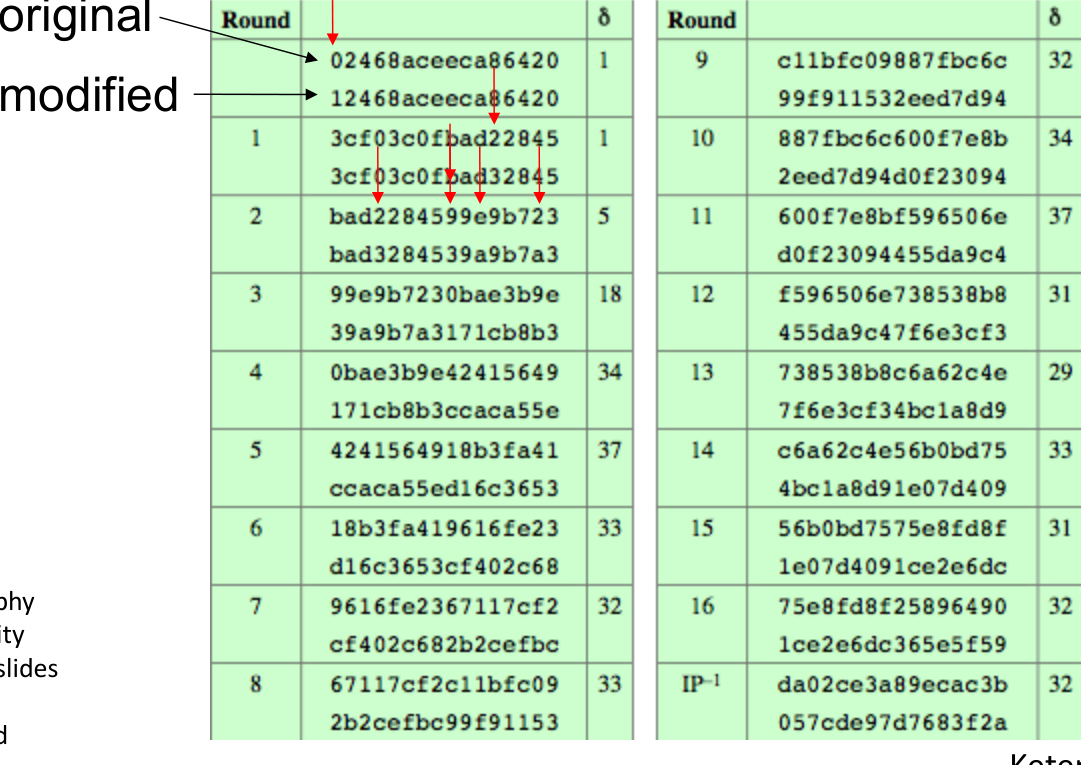
\includegraphics[width=118.23mm,height=210.28mm]{../../images/llm/page_033_img_01.png}%
\end{textblock*}

\end{document}
